\section{Feldman-Cousins comparison with p-theta}
\label{app:fc_compare}

This section presents comparisons of VALOR and p-theta Feldman-Cousins results. In particular \cref{fig:fc_cv_compare} shows the critical values obtained by each group, whilst \cref{app:fc_compare} shows the $2\sigma$ intervals. p-theta excludes inverted hierarchy at $2\sigma$, whilst VALOR has a small region that is not excluded. This difference is driven not by the small differences in critical values in this region, but by the higher inverted hierarchy minimum seen by p-theta with respect to the global minimum (see top row of \cref{fig:fc_interval_compare}). This difference comes from the different templates used by the two fitters; when p-theta uses the same templates as VALOR, better agreement is observed for the contours (see bottom row of \cref{fig:fc_interval_compare}).

\begin{figure*}[htb]
	\center
	\begin{subfigure}[b]{\textwidth}
		\center
		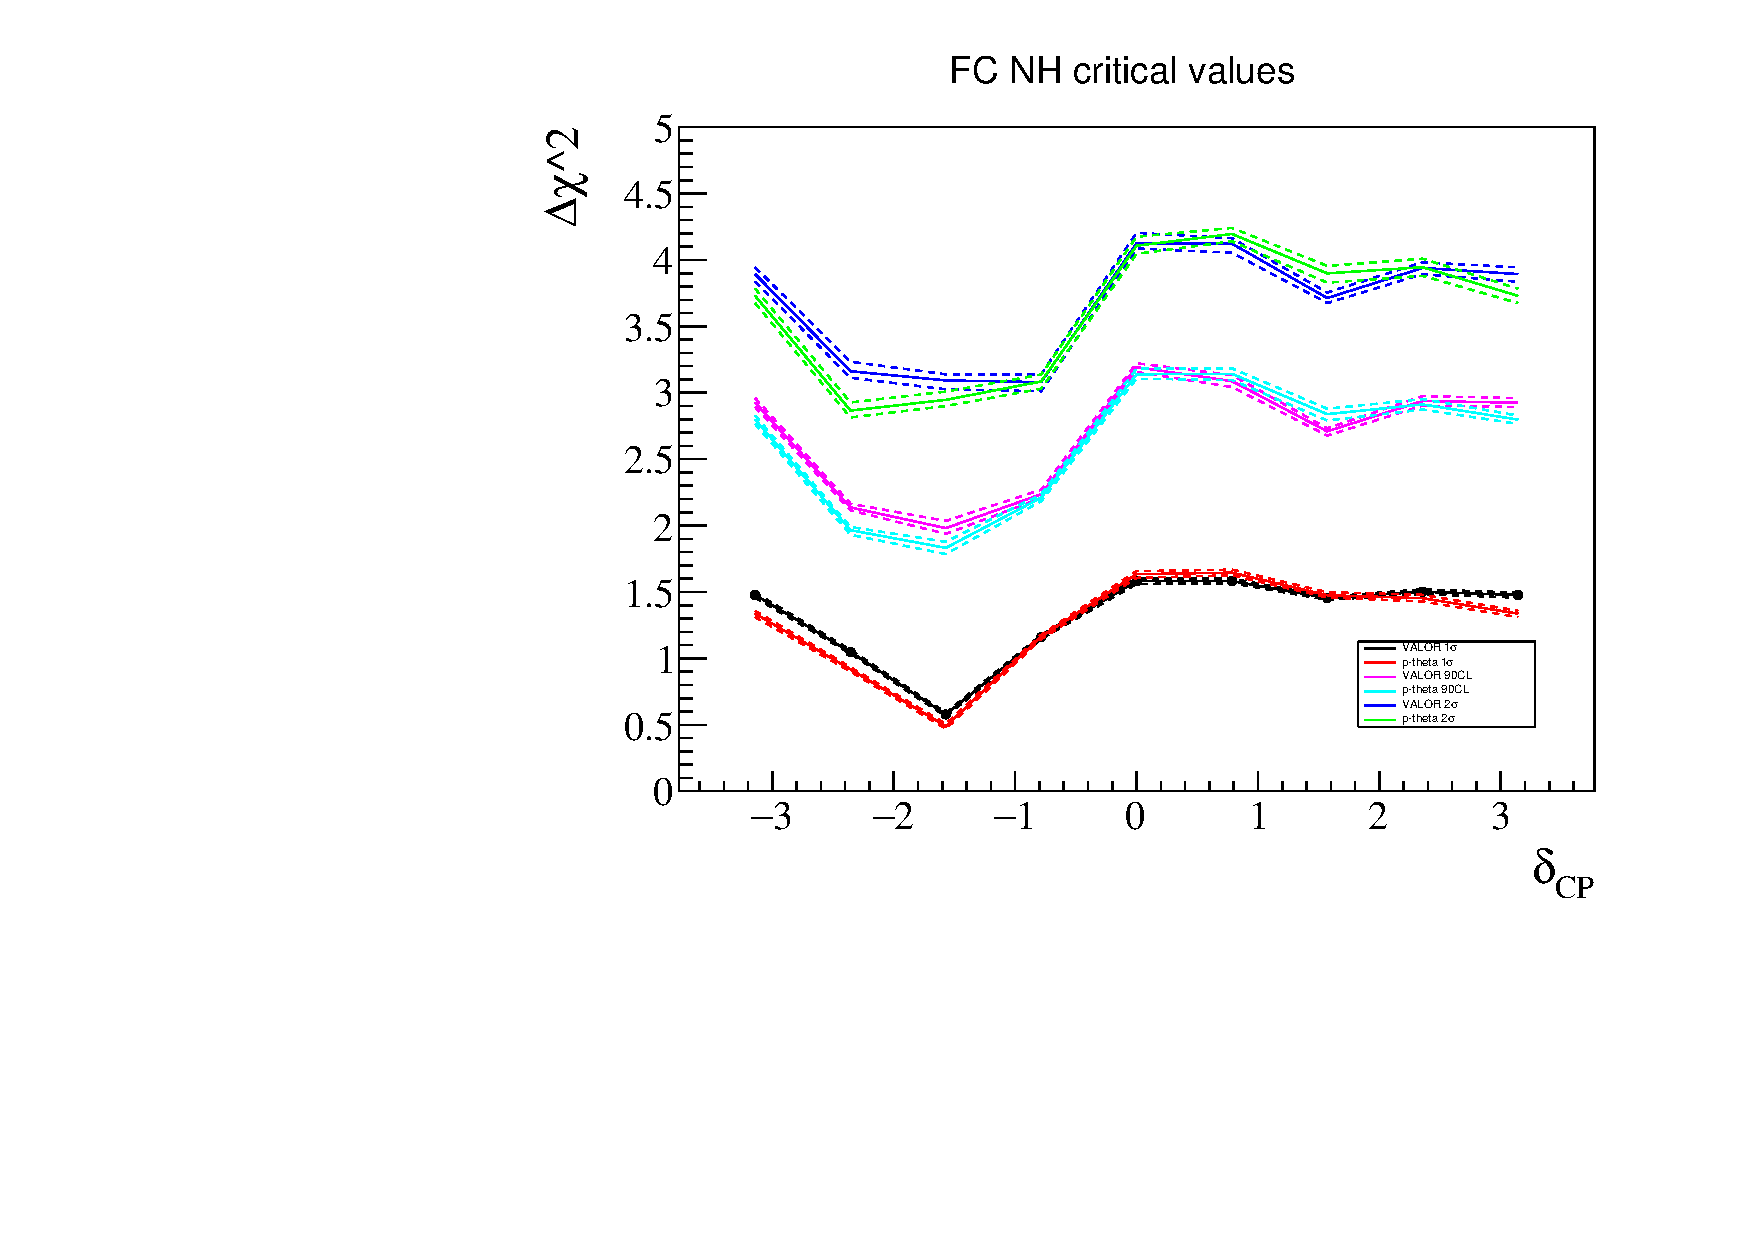
\includegraphics[width=0.68\textwidth, page=1]{images/fc/fc_compare}
		\caption{NH}
	\end{subfigure}
	\begin{subfigure}[b]{\textwidth}
		\center
		\includegraphics[width=0.68\textwidth, page=2]{images/fc/fc_compare}
		\caption{IH}
	\end{subfigure}
	\caption {
		Feldman-Cousins critical values.
	}
	\label{fig:fc_cv_compare}
\end{figure*}

\begin{figure*}[htb]
	\center
	\begin{subfigure}[b]{0.49\textwidth}
		\center
		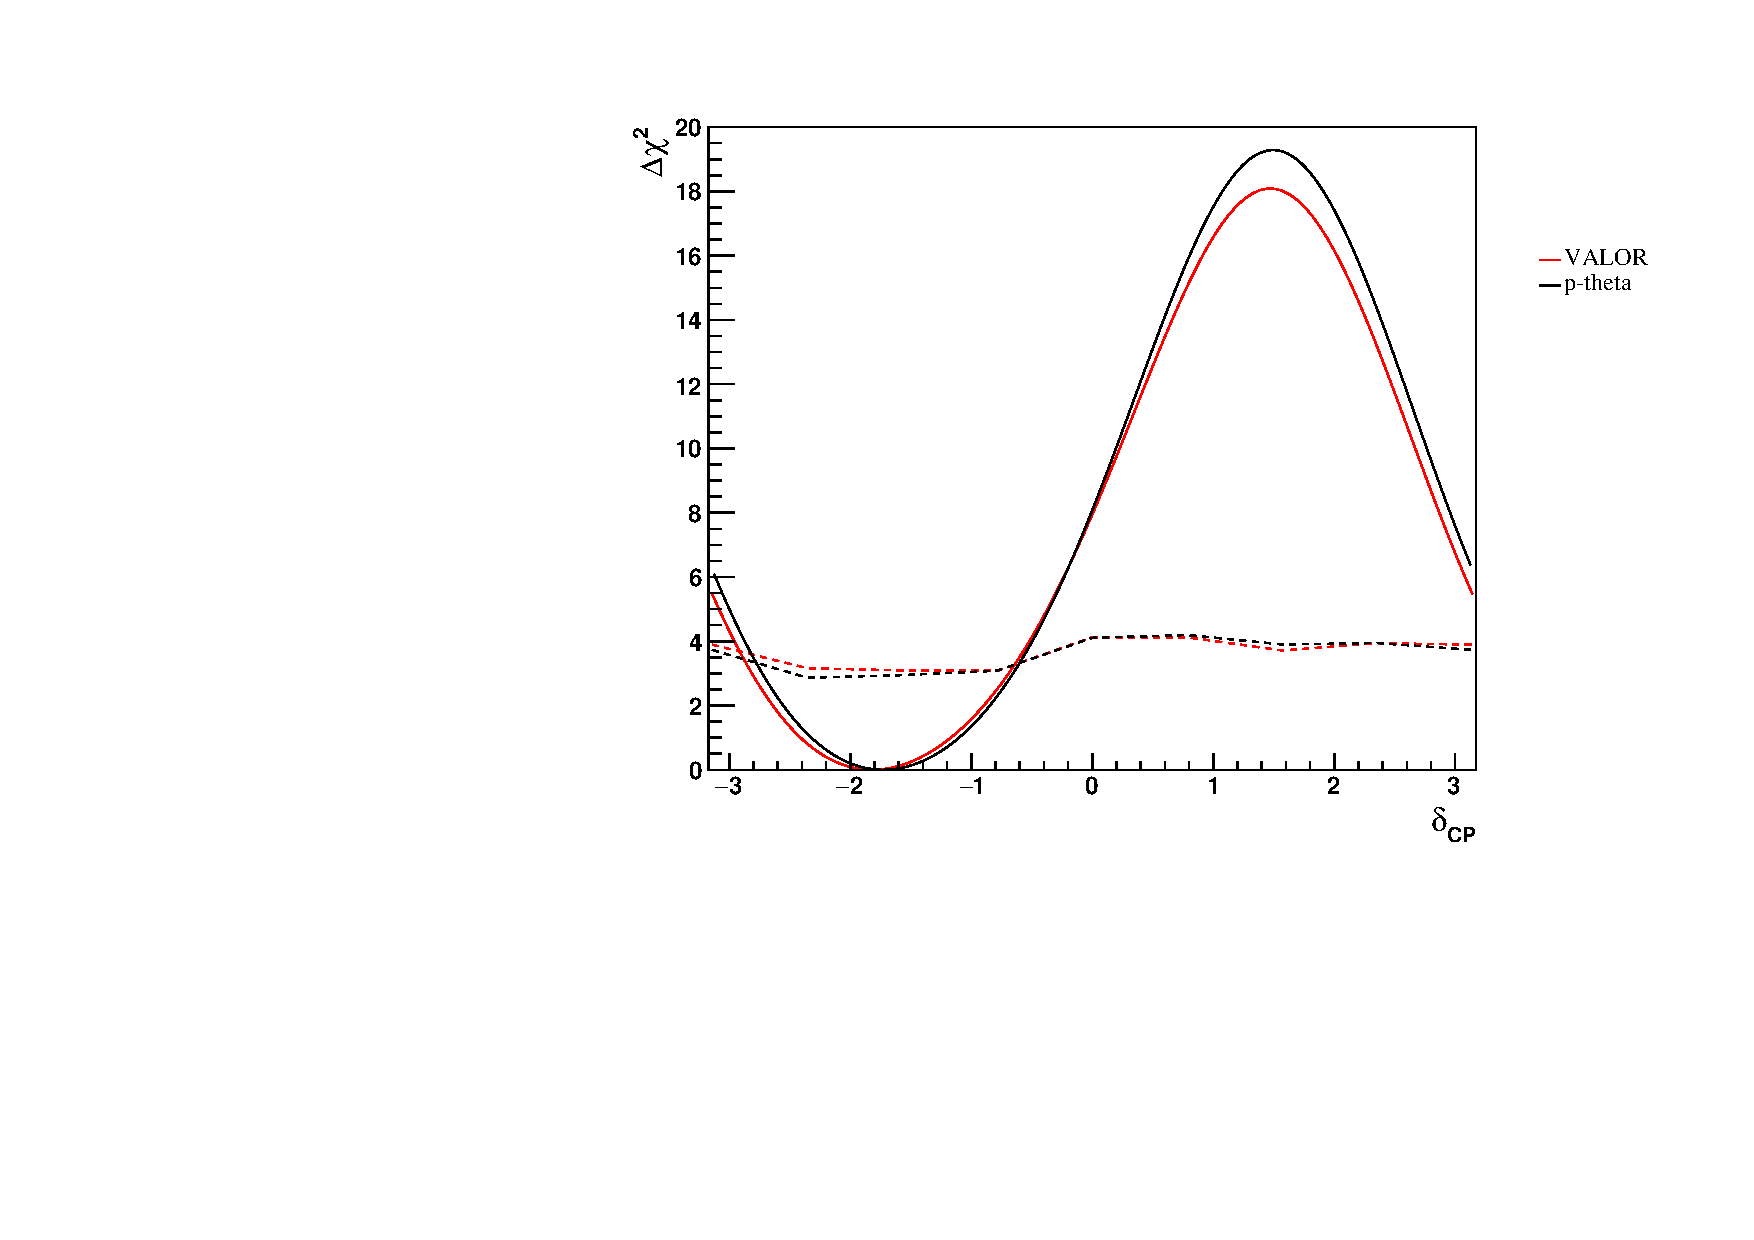
\includegraphics[width=\textwidth]{images/fc/deltacp_fc_nh_global}
		\caption{NH, with p-theta using $p-\theta$ template}
	\end{subfigure}
	\begin{subfigure}[b]{0.49\textwidth}
		\center
		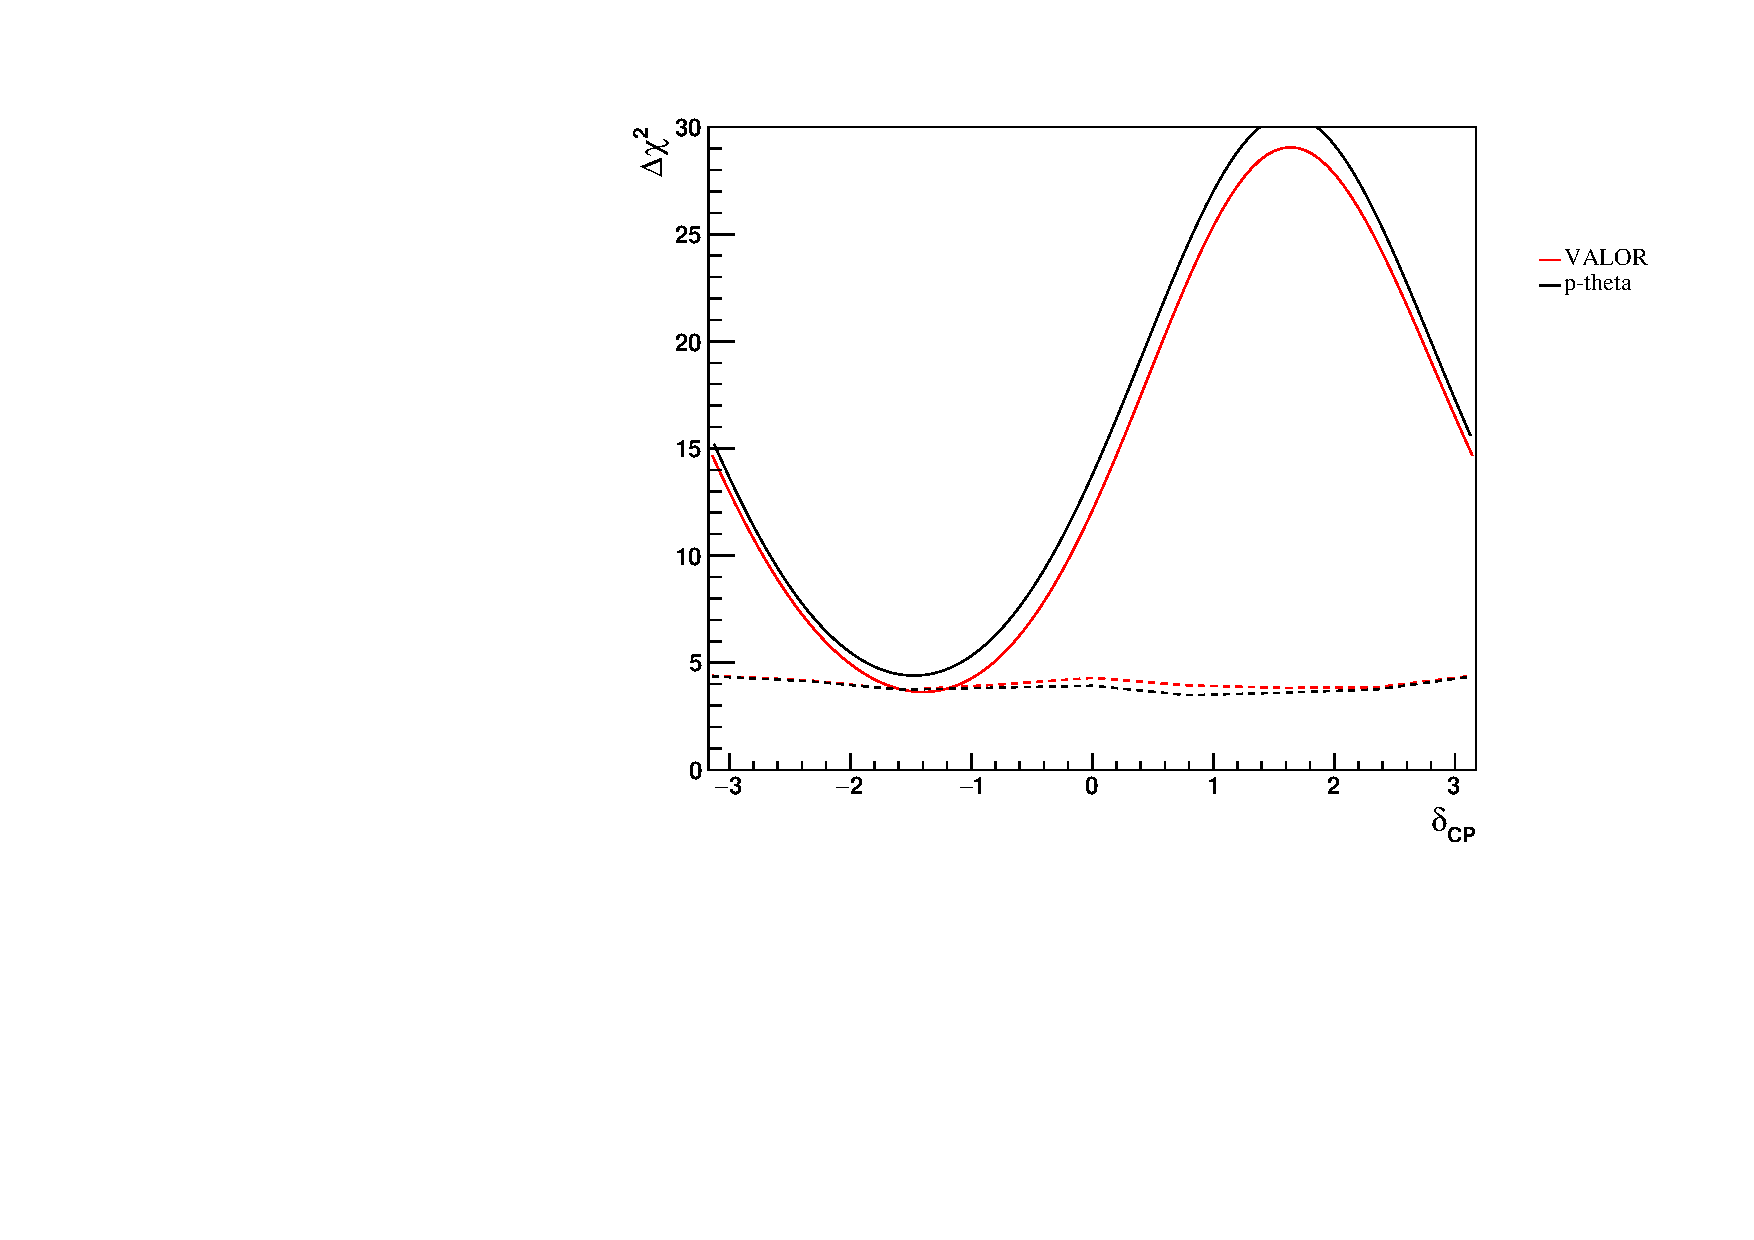
\includegraphics[width=\textwidth]{images/fc/deltacp_fc_ih_global}
		\caption{IH, with p-theta using $p-\theta$ template}
	\end{subfigure}
	\begin{subfigure}[b]{0.49\textwidth}
		\center
		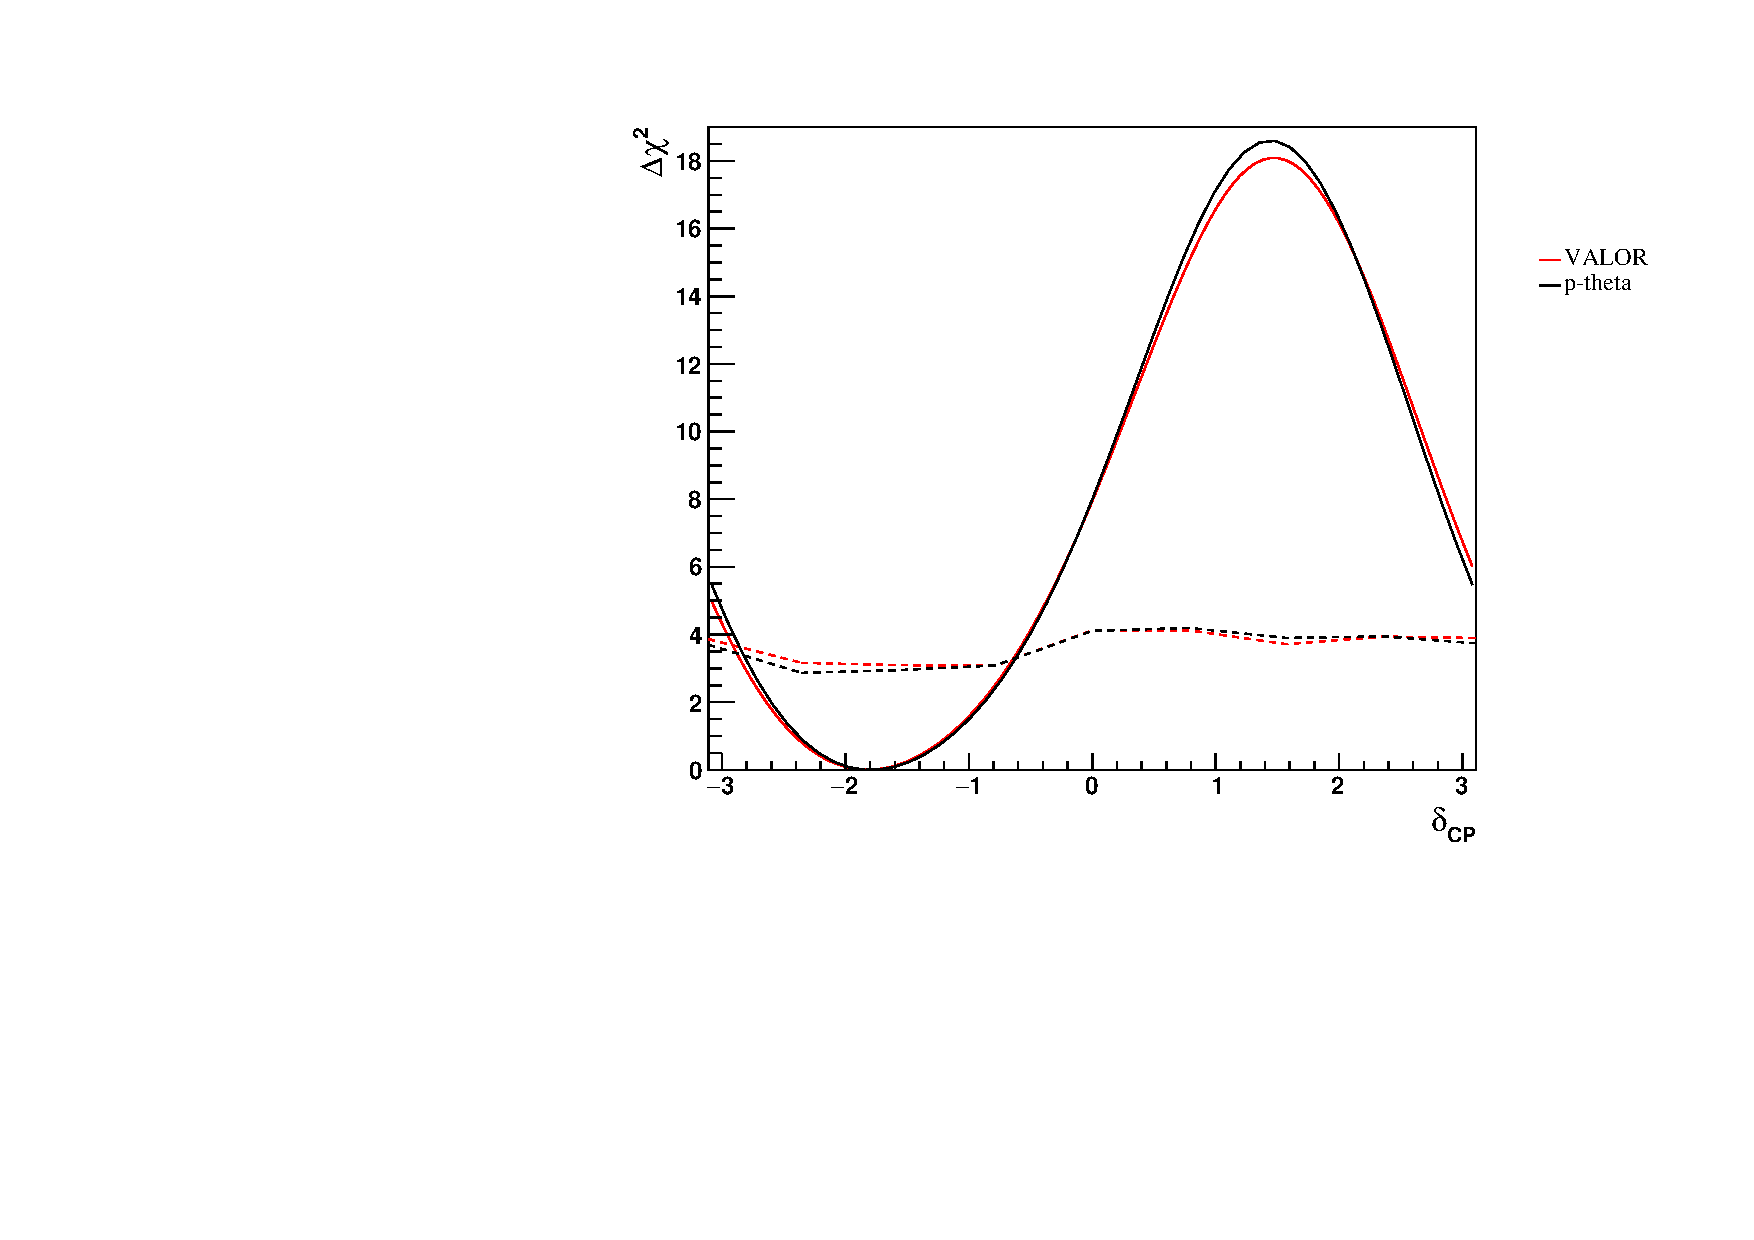
\includegraphics[width=\textwidth]{images/fc/deltacp_wrc_nh_ptheta_erec}
		\caption{NH, with p-theta using $E_r-\theta$ template}
	\end{subfigure}
	\begin{subfigure}[b]{0.49\textwidth}
		\center
		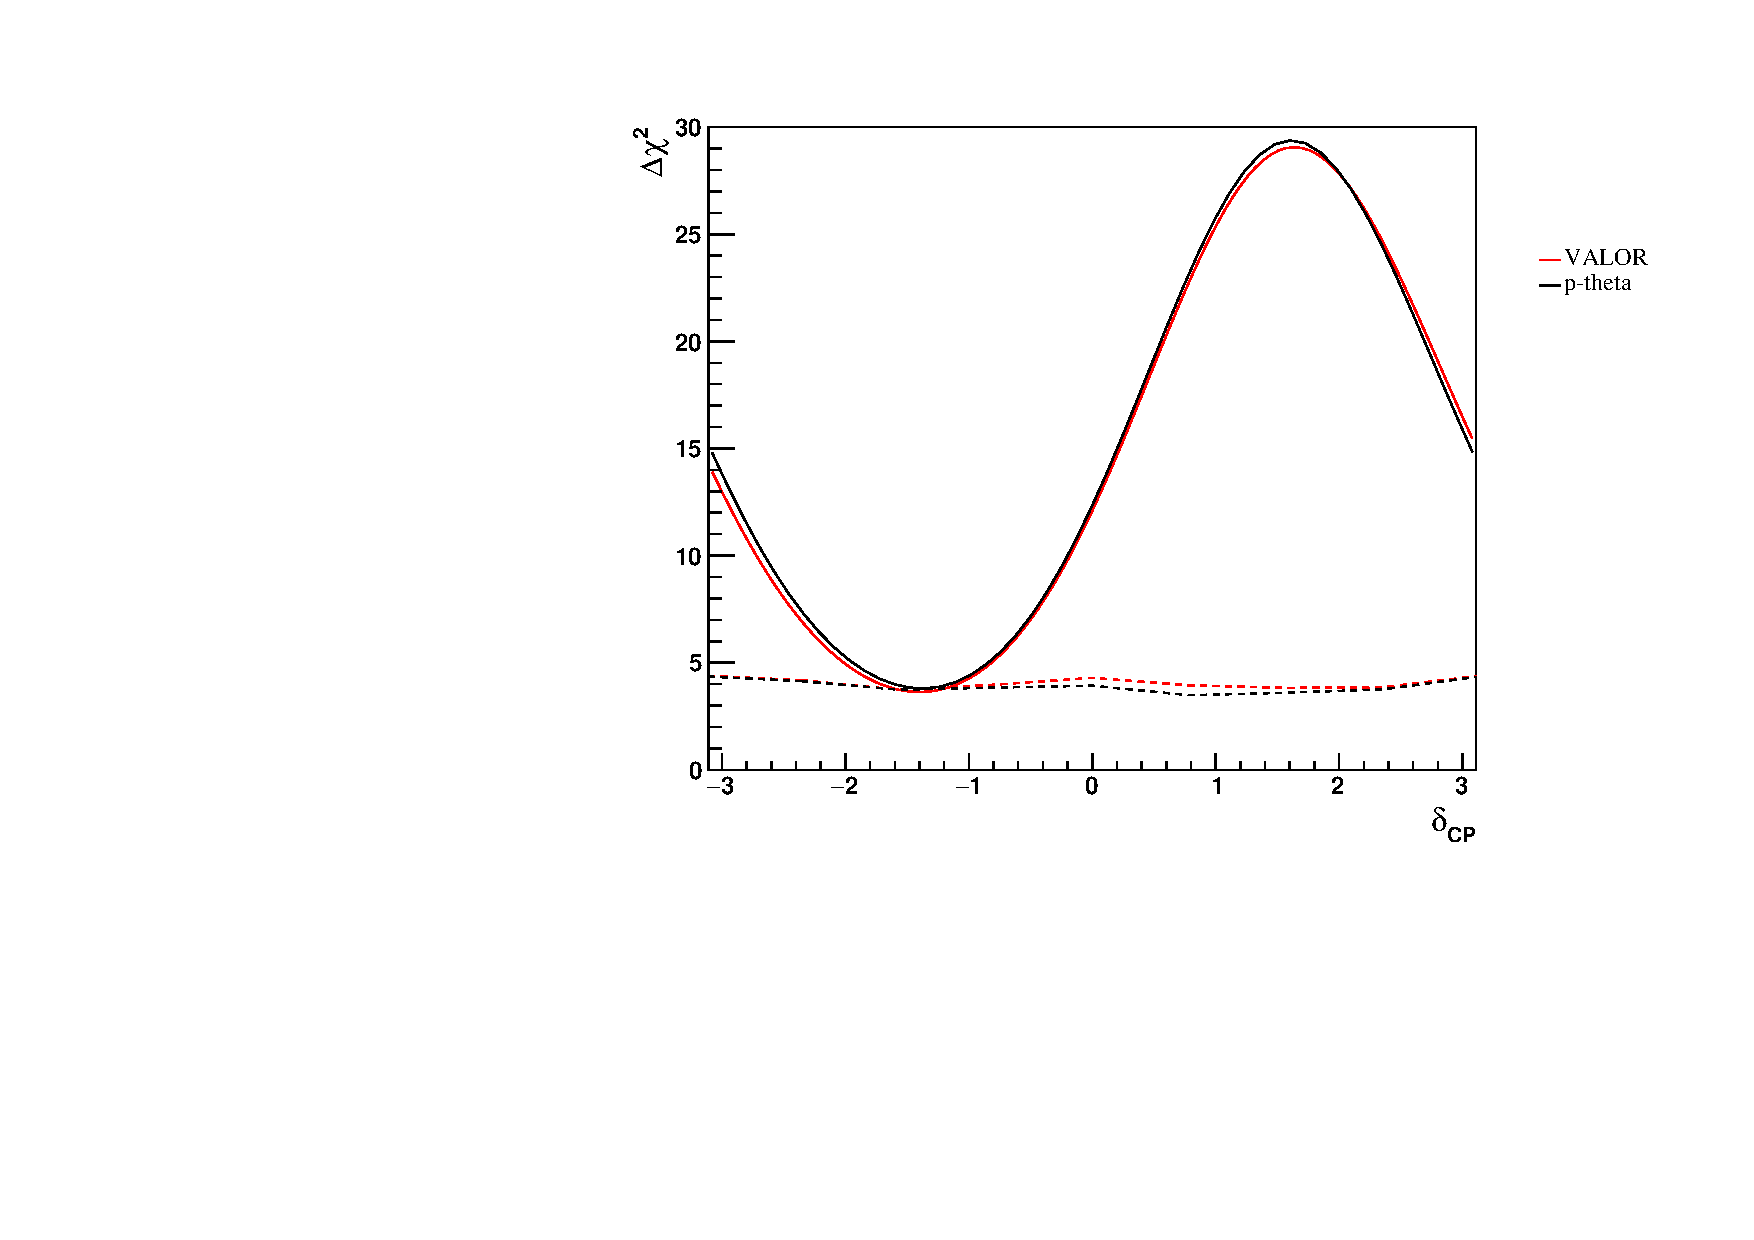
\includegraphics[width=\textwidth]{images/fc/deltacp_wrc_ih_ptheta_erec}
		\caption{IH, with p-theta using $E_r-\theta$ template}
	\end{subfigure}
	\caption {
		\deltacp contours with Feldman-Cousins $2\sigma$ critical values. p-theta contours are computed for $p-\theta$ and $E_r-\theta$ templates, but critical values are only computed for $p-\theta$ templates.
	}
	\label{fig:fc_interval_compare}
\end{figure*}

\clearpage